\documentclass[10pt]{article}

\usepackage[T1]{fontenc}
\usepackage[left=0.82in,right=0.82in,top=0.70in,bottom=0.70in]{geometry}
\usepackage{amsmath,amssymb,mathtools}
\usepackage{booktabs,tabularx,array}
\usepackage{enumitem}
\usepackage{graphicx}
\usepackage{placeins}
\usepackage{xcolor}
\usepackage{hyperref}
\usepackage{microtype}

\hypersetup{
  colorlinks=true,
  linkcolor=blue!45!black,
  citecolor=blue!45!black,
  urlcolor=blue!45!black
}

\setlength{\emergencystretch}{3em}
\setlist[enumerate]{topsep=3pt,itemsep=2pt,leftmargin=1.6em}
\setlist[itemize]{topsep=3pt,itemsep=2pt,leftmargin=1.5em}
\newcommand{\Gref}{G_{\mathrm{ref}}}
\newcommand{\Gint}{G_{\mathrm{int}}}
\newcommand{\dd}{\,\mathrm d}

\title{Paper Dataset Generation:\\
An End-to-End Account}
\author{}
\date{9 August 2026}

\begin{document}
\maketitle

\begin{abstract}
This note follows one case from a random seed to the arrays read by the
trainer.  The replacement dataset contains four kinds of periodic water-wave
states: Stokes waves, Tanaka-profile sums, Benjamin--Feir perturbations, and
JONSWAP/TMA random seas.  Every label is computed with the same fixed
discrete Dirichlet--Neumann operator.

A draw must first lie in the stated parameter range of its family.  A
time-dependent draw is then retained only if its declared fixed-step
calculation returns a complete finite trajectory and keeps the free surface
above the bottom.  Benjamin--Feir revision 4 and JONSWAP/TMA revision 4 trajectories
must also conserve their full internal-band Hamiltonian to relative error at
most \(10^{-3}\) over the autonomous saved-time grid.  No rule based on visual
roughness, sign changes, slope, or model error removes a case.  This document
specifies the replacement dataset.  The source-authenticated release is
complete at 16384 training, 1024 validation, and 1024 test cases per family:
73728 accepted cases from 74045 attempts, 317 zero-row rejections, and
7686144 retained rows.  No reported model has been trained on this release.
\end{abstract}

\section{Objects and guiding rules}

The horizontal interval is $0\leq x<L$, with periodic endpoints and
$L=2\pi$, and gravity is set to one.  A \emph{case} is one sampled initial
surface elevation $\eta_0(x)$, one sampled value $\xi_0(x)$ of the velocity
potential at the surface, and one fixed water depth $h>0$.  A
\emph{trajectory} is the computed evolution of that case.  A \emph{row} is
one retained time from an accepted case.

The case, rather than the row, is the unit of splitting, rejection, and
training weight.  This matters because an accepted Stokes case stores one
row, whereas accepted Tanaka and Benjamin--Feir cases each store 200 rows.
Counting all stored rows equally would therefore give a long trajectory much
more influence than a static wave.

The construction follows four elementary rules.
\begin{enumerate}
  \item Fix the numerical meaning of a label before sampling any cases.
  \item Assign a case to training, validation, or test before seeing whether
        its numerical calculation succeeds.
  \item Replace a failed attempt only within its original parameter category.
  \item Select stored times only after the entire case has been accepted.
\end{enumerate}

\section{The common numerical label}
\label{sec:target}

For given $\eta$, $\xi$, and $h$, let $\varphi(x,y)$ solve
\begin{equation}
  \varphi_{xx}+\varphi_{yy}=0,\qquad
  \varphi_y(x,-h)=0,\qquad
  \varphi(x,\eta(x))=\xi(x).
\end{equation}
Subscripts denote partial derivatives.
The physical Dirichlet--Neumann operator is
\begin{equation}
  G(\eta;h)\xi
  =\left(\varphi_y-\eta_x\varphi_x\right)_{y=\eta(x)}.
  \label{eq:physical-dno}
\end{equation}
It is the slope-corrected upward derivative of the solution $\varphi$ at the
free surface.  In the Zakharov equations it is also $\eta_t$, the
instantaneous rate of change of the surface.

The dataset does not claim to evaluate \eqref{eq:physical-dno} exactly.
Instead, it freezes one discrete reference calculation.  All fields use
$N=1024$ equally spaced points
$x_\ell=2\pi\ell/1024$, $\ell=0,\ldots,1023$.  Since the period is $2\pi$,
the Fourier wavenumbers are the integers.  Let $P_{128}$ discard all modes with
$|k|>128$, and let $P_{128}^{\circ}$ additionally remove the spatial mean.
Let $\mathcal G_{6}^{1024,8}$ denote the implemented order-six
Craig--Sulem calculation on 1024 points with padding factor eight.  The label
is
\begin{equation}
  \boxed{
  \Gref(\eta;h)\xi
  =
  P_{128}^{\circ}\!\left[
    \mathcal G_{6}^{1024,8}
      (P_{128}\eta;h)(P_{128}\xi)
  \right].}
  \label{eq:reference-target}
\end{equation}
The calculation is performed in 64-bit arithmetic.  Only the final spatial
arrays are converted to 32-bit form for storage.  Thus every retained row is
\begin{equation}
  \left(
    P_{128}\eta(t),\
    P_{128}\xi(t),\
    h,\
    t,\
    \Gref(\eta(t);h)\xi(t)
  \right).
  \label{eq:stored-row}
\end{equation}
The model is trained to reproduce the fixed discrete quantity in
\eqref{eq:reference-target}.  Approximation of the continuum operator
\eqref{eq:physical-dno} is a separate question requiring convergence tests
in truncation order, grid size, and padding.
Every constructor removes the spatial mean of $\xi$; this fixes the
irrelevant freedom to add a constant to the potential.

JONSWAP/TMA is evolved on 2048 points, whereas every stored row has 1024
points.  For an $N'$-point field, define the normalized Fourier coefficient
\begin{equation}
  \widehat f_k^{(N')}
  =\frac1{N'}\sum_{j=0}^{N'-1}
    f\!\left(\frac{2\pi j}{N'}\right)e^{-2\pi i jk/N'}.
  \label{eq:normalized-grid-transfer}
\end{equation}
At a retained JONSWAP/TMA time, the program copies the coefficients of
\(\eta\) and \(\xi\) with \(|k|\le128\) from the 2048-point grid, reconstructs
those two fields on 1024 points, and evaluates
\eqref{eq:reference-target} there.  It never resamples the internal
\(G(\eta;h)\xi\): the stored target is recomputed because it is defined by the
1024-point order-six calculation.

\section{One case from beginning to end}
\label{sec:pipeline}

The complete production path is:
\begin{enumerate}
  \item Assign a family, family revision, parameter category, data split, and
        deterministic random-number key, then draw and record all
        initial-condition parameters.
  \item Check the family's stated parameter rules and construct
        $(\eta_0,\xi_0,h)$.  Before rollout, the assembled initial arrays
        must be finite, \(h>0\), and \(h+\eta_0>0\) on the grid.
  \item For a Stokes case, evaluate \eqref{eq:reference-target} at $t=0$.
        For Tanaka and Benjamin--Feir, run the autonomous fixed-step
        calculation in Section~\ref{sec:rollout}.  For JONSWAP/TMA, first run
        its declared nonlinear adjustment, hand its full internal-band
        endpoint to the autonomous solver, and restart the production clock
        at zero.
  \item Apply the whole-case decision in Section~\ref{sec:rollout}.  A failed
        trajectory contributes no rows, including no apparently good prefix.
  \item After acceptance, choose the retained times and write their arrays,
        numerical diagnostics, and checksum.
  \item Count an accepted case toward its original parameter category.  If it
        failed, draw a new case in that same category.
  \item When every family and split quota is complete, build a checked index
        into the array files and pass that index to the trainer.
\end{enumerate}
There are only two case-level gates: membership in the family's declared
construction support, followed by a complete admissible calculation on the
requested interval.  A declared support failure contributes zero rows.  It
is distinct from an unexpected construction or implementation error, which
stops the run.
The sampled specification is written before numerical work, so an
interrupted case can be replayed without drawing a replacement.  An
unexpected construction error, including failure of the initial-array
conditions above, stops the run; it is not silently relabeled as an ordinary
rejected draw.  The declared JONSWAP/TMA phase-realization check is the
exception: nonfinite assembled fields or a nonpositive realized water column
produce a recorded zero-row construction rejection for that case, which is
replaced in the same category while valid batch companions continue.  Other
unclassified constructor failures still stop the run.  Checksums detect
missing or changed array files.

\section{How the four initial-condition families are sampled}
\label{sec:families}

A \emph{parameter category} is a pre-set part of one family's parameter
range that receives its own accepted-case count.  The categories keep important
regimes from disappearing by chance.  Uniform sampling on $[a,b]$ means
that every interval of the same length is equally likely.  Log-uniform
sampling means that $\log h$ is uniform.  A uniform simplex split of a
positive number $A$ chooses nonnegative weights $w_j$ with
$\sum_jw_j=1$ and sets the pieces to $Aw_j$.
Unless an endpoint convention is written explicitly, closed brackets describe
the closure of the continuous support.  The ordinary floating-point uniform
draw includes its lower endpoint and excludes its upper endpoint.  Explicit
endpoint conventions in an individual sampling formula---including half-open
phase and center intervals and the mixed open--closed Benjamin--Feir steepness
draw---override that default.  The distinction has probability zero for the
continuous law but is recorded for exact replay.

\begin{table}[ht]
  \centering
  \small
  \caption{The four training families.  A horizon is needed only for a
  time-dependent family.}
  \label{tab:families}
  \begin{tabularx}{\textwidth}{
    @{}>{\raggedright\arraybackslash}p{0.17\textwidth}
       >{\raggedright\arraybackslash}p{0.13\textwidth}
       >{\raggedright\arraybackslash}X
       >{\raggedright\arraybackslash}p{0.15\textwidth}@{}}
    \toprule
    Family & Categories & Main distinction & Horizon / retained rows \\
    \midrule
    Stokes
      & 4
      & finite/deep branch and low/moderate steepness
      & static / 1 \\
    Tanaka
      & 11
      & regime, number of crests, and number moving right
      & $T=200$ / 200 \\
    Benjamin--Feir
      & 66
      & one feasible carrier--sideband integer pair per category
      & last $0.08$-grid time not exceeding $100T_c$ / 200 \\
    JONSWAP/TMA
      & 27
      & shallow/finite/deep, peak enhancement, and direction balance
      & last $0.08$-grid time not exceeding 16 peak periods / 16 \\
    \bottomrule
  \end{tabularx}
\end{table}

\subsection{Fifth-order Stokes states}

A Stokes draw first fixes one of four parameter categories:
\[
  \{\text{finite},\text{deep}\}
  \times
  \{0.005\leq ka<0.03,\quad 0.03\leq ka\leq0.15\}.
\]
Here $k$ is the carrier wavenumber and $a$ is the expansion-amplitude
parameter of the fifth-order formula.  Because the first harmonic receives
nonlinear corrections, $a$ is not exactly the realized first-harmonic
amplitude.  The common parameter interval is
\[
  0.000766\leq a\leq0.011494.
\]
For the finite-depth branch, the mode number is
$n\in\{14,\ldots,26\}$, the wavenumber is $k=n$, and
\[
  0.02\leq h\leq1.5,\qquad 0.5\leq kh\leq5.
\]
For the deep branch,
\[
  n\in\{1,\ldots,20\},\qquad 4\leq h\leq50,\qquad kh\geq5.
\]
The branch is assigned before \(n\) and \(h\) are drawn.  Thus the shared
boundary \(kh=5\) does not select a formula: a finite-category case uses the
finite-depth coefficients and a deep-category case uses the deep-water
coefficients.  Allowing equality in both branch-specific supports therefore
creates no ambiguous case record.
The program lists the modes compatible with the chosen category and selects one
uniformly.  It then draws $h$ log-uniformly in the compatible depth interval,
draws a phase $\phi$ uniformly on $[0,2\pi)$, and draws $a$ uniformly from the
intersection of the common amplitude interval and the chosen $ka$ interval.
The code evaluates Fenton's fifth-order analytic Stokes expansion, using its
finite-depth coefficients or deep-water limit, to construct
$(\eta_0,\xi_0)$~\cite{fenton1985}.  The parameter ranges, four parameter
categories, random phase, and depth law above are dataset choices rather than
claims made by Fenton.

The finite-depth formula is used only in its intended Stokes regime.  For
phase $\theta=kx+\phi$, write its elevation as
\[
  \eta_5(\theta)=\sum_{r=1}^{5}E_r\cos(r\theta),
\]
where $E_r$ is the coefficient of harmonic $r$.  Let $H_{4096}$ be the
largest sampled value of $\eta_5$ minus its smallest sampled value on 4096
equally spaced phases, and define
\[
  H_+
  =
  H_{4096}
  +\frac14\left(\frac{2\pi}{4096}\right)^2
    \sum_{r=1}^{5}r^2|E_r|.
\]
The last term bounds the possible height missed between two phase samples.
With wavelength $\lambda=2\pi/k$, the required support condition is
\begin{equation}
  \mathrm{Ur}_+
  =\frac{H_+\lambda^2}{h^3}
  \leq26.
  \label{eq:ursell}
\end{equation}
This is a conservative Ursell-number restriction for the fifth-order
formula, not a fitted predictor of whether a numerical rollout would
survive~\cite{fenton1985,zhao2024}.  If \eqref{eq:ursell} fails, the mode,
depth, phase, and parameter category remain fixed and only the amplitude is
redrawn, with at most 1000 redraws.  Exhausting that limit gives a zero-row
attempt, and the category receives a new case.  A valid Stokes case is static:
it stores only \eqref{eq:stored-row} at $t=0$.

\subsection{Periodic Tanaka-profile sums}

The three main Tanaka structural groups contain $m=1,2,3$ component profiles.
First draw their total dimensionless amplitude
\[
  A\sim\operatorname{Unif}[0.10,0.35].
\]
Next draw
$(W_1,\ldots,W_m)\sim\operatorname{Dirichlet}(1,\ldots,1)$ and set
\[
  \alpha_j=AW_j,
  \qquad j=1,\ldots,m.
\]
For $m=1$, $W_1=1$.  Hence $\alpha_j$ is the amplitude-to-depth ratio of
component $j$ and $\sum_j\alpha_j=A$.

Depth is drawn after the amplitudes.  Define the largest component ratio and
its inverse-width proxy by
\begin{equation}
  \alpha_{\max}=\max_j\alpha_j,
  \qquad
  \kappa_{\max}=\frac{\sqrt{3\alpha_{\max}}}{2h}.
  \label{eq:tanaka-kdv-scale}
\end{equation}
The expression for $\kappa_{\max}$ is the inverse-width scale in the
small-amplitude KdV solitary-wave formula.  We use it only as an elementary
resolution proxy for the narrowest requested crest; it is not the exact
width of a finite-amplitude Tanaka wave.  Since the delivered band ends at
$|k|=128$, define
\begin{equation}
  R=\frac{128}{\kappa_{\max}}.
  \label{eq:tanaka-resolution-ratio}
\end{equation}
The revision-3 support requires $R\geq10$.  Equivalently, set
\begin{equation}
  h_{\min}
  =\max\!\left\{
    h_{\mathrm{base}},
    \frac{10\sqrt{3\alpha_{\max}}}{256}
  \right\},
  \qquad
  h=h_{\min}^{1-U_h}h_{\max}^{U_h},
  \qquad
  U_h\sim\operatorname{Unif}[0,1].
  \label{eq:tanaka-conditional-depth}
\end{equation}
The main groups use $h_{\mathrm{base}}=0.01$ and $h_{\max}=0.30$.
The steep structural group has one crest and uses
$A=\alpha_1\sim\operatorname{Unif}[0.25,0.45]$,
$h_{\mathrm{base}}=0.20$, and $h_{\max}=0.35$.  For every steep amplitude,
the second entry in the maximum in \eqref{eq:tanaka-conditional-depth} is
less than $0.20$.  Thus the conditional lower bound is inactive there and
the steep depth remains the geometric interpolation from $0.20$ to $0.35$.

At fixed amplitudes, uniform $U_h$ makes $\log h$ uniform on the declared
interval.  This gives equal increments of multiplicative profile scale; it
is a numerical coverage rule, not a probability model for physical depths.

Let $s_j\in\{-1,+1\}$ denote the direction of crest $j$, with $s_j=+1$
for rightward travel, and let
\[
  q=\#\{j:s_j=+1\}
\]
be the number of right-moving crests.  For a main case, each pair $(m,q)$
with $m\in\{1,2,3\}$ and $q=0,\ldots,m$ is a parameter category.  These give
$2+3+4=9$ categories.  The steep one-crest group contributes the two
categories $q=0,1$, for eleven Tanaka categories in total.  Conditional on
$q$, the sampler chooses uniformly which $q$ of the $m$ exchangeable crest
labels move right; the rest move left.

The accepted-case quota is divided as evenly as possible across all eleven
categories.  Therefore the distinct direction compositions receive equal
coverage, rather than the binomial frequencies generated by independent fair
signs.  Left and right directions remain balanced marginally in the ideal
equal-category population.  For a finite quota, category counts differ by at
most one and a one-case direction imbalance is possible; the fixed order gives
a quota of 1024 one extra left-moving one-crest case.  Because the one-, two-,
and three-crest main groups contain two, three, and four direction
compositions, their aggregate shares are $2/11$, $3/11$, and $4/11$; the
steep group has share $2/11$.  This deliberately replaces the old four-group
independent-sign mixture.

The direction categories were introduced in Tanaka revision 2.  Revision 3
retains all eleven categories but draws amplitudes before depth and uses
\eqref{eq:tanaka-conditional-depth}.  A revision-2 proposal remains exactly
replayable, but it cannot be resumed into a revision-3 run.  Benjamin--Feir
and JONSWAP/TMA use revision 4, and static Stokes remains at revision 2.

The value 10 was fixed by a full-horizon boundary calculation with
$\alpha\in\{0.225,0.30,0.35\}$, $R\in\{6,8,10\}$, and internal cutoffs
$J\in\{224,256\}$.  For the cutoff-$J$ history, define
\[
  d_J(t)=P_{128}^{\circ}\!\left[
    \mathcal G_6^{1024,8}(\eta_J(t);h)\xi_J(t)
  \right]
  -G_{\mathrm{ref}}(P_{128}\eta_J(t);h)P_{128}\xi_J(t)
\]
and
\[
  C_J=
  \frac{\max_t\lVert d_J(t)\rVert_{2,N}}
       {\max_s\lVert
         G_{\mathrm{ref}}(P_{128}\eta_J(s);h)P_{128}\xi_J(s)
       \rVert_{2,N}+10^{-12}},
\]
where $\lVert\cdot\rVert_{2,N}$ is the root-mean-square norm on the spatial
grid.  The reported statistic is $\max_{J\in\{224,256\}}C_J$.  Its worst
values were $2.91\times10^{-3}$ at $R=6$, $6.31\times10^{-4}$ at $R=8$,
and $1.40\times10^{-4}$ at $R=10$.  Thus $R=6$ exceeded the $10^{-3}$ budget,
whereas $R=8$ passed with little margin.  Directly comparing the same
cutoff-$224$ and cutoff-$256$ histories gave the same ordering: $R=6$ failed,
while the worst delivered-field discrepancies at $R=8$ and $R=10$ were
respectively $7.34\times10^{-4}$ and $1.35\times10^{-4}$.  We therefore use
the conservative value 10 rather than the merely passing value 8.

The centers are periodic and separated.  Draw nonnegative simplex weights
$w_j$ with $\sum_jw_j=1$ and set the cyclic gaps to
\begin{equation}
  d_j=3h+(2\pi-3mh)w_j.
  \label{eq:tanaka-gaps}
\end{equation}
The gaps sum to $2\pi$ and are all at least $3h$.  A common uniform rotation
on the periodic interval then fixes the centers $x_j$ without favoring
$x=0$.

For each requested amplitude ratio $\alpha$, the code numerically solves a
unit-depth permanent-form solitary wave using Tanaka's
formulation~\cite{tanaka1986}.  Xu and Guyenne used the same solitary-wave method for
their long-time finite-depth test~\cite{xu2009}.  Let $\Phi$ be the
surface-potential coordinate used in the solve, $X$ the dimensionless
horizontal coordinate, $Q=e^\tau$ the fluid-speed magnitude, $\tau$ its
logarithm, $\theta$ the angle of the free-surface tangent, and $F_\alpha$ the
resulting Froude number.  The code adjusts the crest value of $Q$ by bisection
until the reconstructed crest height is $\alpha$, iterates Tanaka's
relations, and reconstructs the dimensionless elevation
$\bar\eta_\alpha$ from
\[
  \frac{\dd X}{\dd\Phi}=\frac{\cos\theta}{Q},
  \qquad
  \frac{\dd\bar\eta_\alpha}{\dd\Phi}
  =\frac{\sin\theta}{Q}.
\]
It uses 257 uniformly spaced nodes on \(0\leq\gamma\leq2.5\), reflects them
about zero to obtain 513 nodes, and applies the project-fixed map
\(\Phi=0.01\gamma+\gamma^5\).  It performs 80 fixed-point updates.  These
discretization choices are ours; they are not parameters prescribed by
Tanaka.

Before interpolation, the constructor verifies that both endpoint elevations
and the endpoint and crest tangents differ from zero by at most $10^{-12}$,
then sets those quantities exactly to zero.  The corrected values and tangents
are joined by cubic Hermite interpolation, then extended by zero with
continuous value and first derivative.  Every
periodic copy that intersects the domain is included.  This compact
extension, Hermite placement, periodization, multi-crest superposition, and
spectral projection are project construction choices.  In particular, a sum
of profiles is an initial condition made from Tanaka solitary waves, not an
exact steady multi-soliton solution.
For component $j$,
\begin{equation}
  \eta_j(x)
  =
  h\sum_{r\in\mathbb Z}
  \bar\eta_{\alpha_j}
  \!\left(\frac{x-x_j+2\pi r}{h}\right).
  \label{eq:tanaka-elevation}
\end{equation}
Only finitely many terms are nonzero.  The interpolation is evaluated first
on an eight-times finer grid and then restricted to the 1024-point grid.

Set $c_j=F_{\alpha_j}\sqrt{gh}$, with $g=1$ in this dataset, and define
\begin{equation}
  \rho_j(x)
  =
  \bigl(1+\eta_{j,x}(x)^2\bigr)
  \bigl(c_j^2-2\eta_j(x)\bigr).
  \label{eq:tanaka-radicand}
\end{equation}
The following conversion of the traveling profile into the project's
periodic Zakharov variables is not quoted as an equation from Tanaka.  The
candidate derivative of the surface potential is
\[
  r_j(x)=s_j\bigl[c_j-\sqrt{\rho_j(x)}\bigr].
\]
A periodic antiderivative exists after subtracting the spatial mean of
$r_j$.  The program therefore defines $\xi_j$ by
\[
  \partial_x\xi_j=r_j-\frac1{2\pi}\int_0^{2\pi}r_j(x)\,\dd x,
  \qquad
  \int_0^{2\pi}\xi_j(x)\,\dd x=0,
\]
using Fourier division by $ik$ on every nonzero mode.  Finally,
\[
  (\eta_0,\xi_0)
  =
  P_{128}\sum_{j=1}^{m}(\eta_j,\xi_j).
\]
This sharp projection is applied once before rollout; the result is then
zero-filled into the $K=256$ evolution band.  Modes
$129\leq |k|\leq256$ are therefore zero initially but may be generated by
nonlinear evolution.
A finite negative value of $\rho_j$ is outside this construction and yields a
zero-row attempt; it is never clipped to zero.  A nonfinite value or an
invalid wave speed signals a construction error and stops generation rather
than being silently redrawn.

\subsection{Benjamin--Feir carrier and sidebands}

This family uses depth $h=5$.  Let $\epsilon_c$ denote the steepness of the
first carrier-elevation harmonic, and let $\rho$ denote the amplitude of each
first-harmonic sideband divided by the amplitude of that carrier harmonic.
Choose a carrier mode
$n_c\in\{4,\ldots,20\}$ and a positive sideband separation
$\Delta n<n_c$.  Define the normalized sideband location
\begin{equation}
  \beta
  =\frac{\Delta n/n_c}{2\sqrt2\,\epsilon_c}.
  \label{eq:bf-condition}
\end{equation}
Benjamin and Feir give the historical deep-water instability
condition~\cite{benjaminfeir1967}.  In the present normalization,
equation~(4.6) of Andrade and Stuhlmeier gives
$0<\beta<1$~\cite{andrade2023}.  Exactly 66 integer pairs
$(n_c,\Delta n)$ can intersect this band for
$0.05\leq\epsilon_c\leq0.13$; each pair is one parameter category.

Equations~(5.7)--(5.11) of Andrade and Stuhlmeier give the
Akhmediev-breather correspondence and the focused-envelope amplification
factor $1+2\sqrt{1-\beta^2}$ in this normalization.  We therefore define the
scalar screening proxy
\begin{equation}
  \epsilon_f
  =\epsilon_c\left(1+2\sqrt{1-\beta^2}\right)
  \label{eq:bf-focused-steepness}
\end{equation}
and use the pre-rollout support
\begin{equation}
  0<\beta<1,\qquad
  \epsilon_f\leq F_0,\qquad
  F_0=\frac{1+\sqrt2}{10},\qquad
  0.05\leq\rho\leq0.10.
  \label{eq:bf-focused-support}
\end{equation}
The value $F_0$ is the value of \eqref{eq:bf-focused-steepness} at the
moderate reference steepness $\epsilon_c=0.10$ and the leading-NLS
maximum-growth location $\beta=1/\sqrt2$.  It is our population choice, not
a theorem giving a wave-breaking or regularity boundary.  Yang and Liu use
$\epsilon_c=0.10$, five-percent sidebands, and the maximum-growth frequency
coordinate $\Delta\omega/(\omega_c\epsilon_c)=1$
\cite[Sec.~4.3.1]{yangliu2024}.  Under the leading deep-water narrowband
relation $\Delta k/k_c\simeq2\Delta\omega/\omega_c$, this corresponds to
$\beta\simeq1/\sqrt2$ in our symmetric-wavenumber normalization.  Our
sideband interval joins that five-percent value to the ten-percent
perturbation of Xu and Guyenne~\cite{xu2009}.

For an elementary description of the conditional draw, set
\[
  \ell=\frac{\Delta n}{2\sqrt2\,n_c},\qquad
  \epsilon_{\min}
  =\max\{0.05,\ell\},
\]
and
\[
  \epsilon_{\max}
  =\min\!\left\{0.13,
    \frac{-F_0+2\sqrt{F_0^2+3\ell^2}}{3}\right\}.
\]
The sampler draws
\[
  \epsilon_c\sim
    \operatorname{Unif}(\epsilon_{\min},\epsilon_{\max}],\qquad
  \rho\sim\operatorname{Unif}[0.05,0.10),\qquad
  x_0\sim\operatorname{Unif}[0,2\pi).
\]
The upper endpoint is obtained by solving $\epsilon_f=F_0$ for
$\epsilon_c$ at fixed $(n_c,\Delta n)$.  It ranges from $0.081763$ to
$0.13$ over the 66 categories, so no integer category is removed.  The
relative phase of both sidebands is fixed at $\theta=-\pi/4$.  Changing the
sampled support advances the Benjamin--Feir family revision from 3 to 4.  The
revision-4 family retains the revision-3 numerical evolution method; an old
revision-3 proposal cannot be resumed into a revision-4 output root.

Because the period is $2\pi$, set
$k_c=n_c$, $k_\pm=n_c\pm\Delta n$, and $a=\epsilon_c/k_c$.
$a$ is the amplitude of the first carrier harmonic; $\epsilon_c$ is not
computed from half the total crest-to-trough height.
Let $(\eta_c,\xi_c)$ be the fixed and recorded fifth-order deep-water Stokes
carrier, put $y=x-x_0$, and set the carrier phase to zero in the translated
coordinate $y$.
The initial state is
\begin{align}
  \eta_0(x)
    &=
    \eta_c(y)
    +\rho a\{\cos(k_-y+\theta)+\cos(k_+y+\theta)\}, \notag\\
  \xi_0(x)
    &=
    \xi_c(y)
    +\rho a\!\left\{
      \sqrt{\frac1{k_-}}e^{k_-\eta_0(x)}\sin(k_-y+\theta)
      +
      \sqrt{\frac1{k_+}}e^{k_+\eta_0(x)}\sin(k_+y+\theta)
    \right\},
  \label{eq:bf-state}
\end{align}
followed by removal of the mean of $\xi_0$ and projection to the delivered
band.  The sidebands follow equation~(33) of Xu and Guyenne, who in turn
followed Dommermuth and Yue~\cite{xu2009,dommermuth1987}.  Their single
published case used
\[
  (n_c,\Delta n,\epsilon_c,\rho,\theta)
  =(9,2,0.13,0.10,-\pi/4)
\]
and a numerically computed steady deep-water carrier.  Our code preserves
their symmetric Airy-sideband formula, fixed relative phase, and use of the
total $\eta_0$ inside both exponentials.  Translating the complete state
changes neither the relative phases nor the quartet phase
$\theta+\theta=-\pi/2$.  The 66 mode-pair categories, randomized parameters,
finite proxy depth $h=5$, and analytic fifth-order carrier are our
generalization, so this is not an exact reproduction of their one initial
state.

Let
\[
  T_c=\frac{2\pi}{\sqrt{k_c}},\qquad
  T_{\mathrm{BF}}
  =0.08\left\lfloor\frac{100T_c}{0.08}\right\rfloor.
\]
The rollout ends at the last saved-grid time not exceeding 100 linear carrier
periods.  Thus $100T_c$ is the intended horizon and
$T_{\mathrm{BF}}$ is its strictly floored saved-grid endpoint.  Across the
66 equally weighted mode-pair categories, $T_{\mathrm{BF}}$ ranges from
$140.48$ to $314.08$ and has mean $174.50$; equivalently,
$T_{\mathrm{BF}}/T_c\in[99.9541,99.9973]$.

This support was frozen before validation stream 934 was numerically
advanced.  That calculation drew one case in each of the 66 mode-pair
categories and evolved every case to the saved-grid endpoint immediately
below its intended $100T_c$ horizon with the numerical method inherited
from revision 3: the state retained Fourier modes $|k|\leq256$, the
internal Dirichlet--Neumann calculation used order four, and the time step
was $0.01$.  All 66 attempts
were accepted and none was replaced.  All 13,200 retained frames were finite;
the largest relative internal-Hamiltonian drift was
$5.38713\times10^{-5}$, the largest implicit-stage residual was
$9.999984\times10^{-9}$, and the smallest water column was $4.958158$.
This is evidence that the declared support is numerically usable under the
tested discretization and horizon.  It does not turn $\epsilon_f$ into the
maximum physical slope or prove regularity of the full water-wave equations;
the complete-trajectory checks in Section~\ref{sec:rollout} therefore remain
mandatory.  Stream 934 is support-validation evidence.  Because it selected
cases by conditioning proposals from the preceding revision-3 law, it is not
the exact-source production gate; that role belongs to revision-4 stream 935,
reported in Section~\ref{sec:release}.

\subsection{Relative-frequency-band JONSWAP/TMA random seas}

Each random-sea parameter category fixes one depth regime, one peak-enhancement value
$\gamma\in\{1,3.3,5\}$, and one right-moving energy fraction
$r_d\in\{0,\tfrac12,1\}$.  This gives $3\cdot3\cdot3=27$ categories.

Let $k_p>0$ be the reference peak wavenumber and let $h>0$ be the depth.
For wavenumber $k>0$, define
\[
  \omega(k,h)=\sqrt{k\tanh(kh)},
  \qquad \omega_p=\omega(k_p,h).
\]
Revision 4 retains frequencies in the interval
$\tfrac12\omega_p\leq\omega\leq\tfrac52\omega_p$.  Phase-resolved numerical
JONSWAP calculations have used exactly this interval~\cite{draycott2026},
and an earlier random-wave calculation used the upper endpoint
$\omega_{\max}=2.5\omega_p$~\cite{grice2015}.  We use it as a finite
component definition, not as a wave-breaking criterion.  Its parameter support
therefore also requires
\begin{equation}
  \omega(128,h)\geq\frac52\,\omega_p.
  \label{eq:jonswap-frequency-fit}
\end{equation}
This ensures that the upper end of the declared relative-frequency interval
fits inside the delivered band.

Let $H_s$ denote significant wave height.  In the shallow regime, choose a
reference peak mode
$n_p$ uniformly from $\{16,18,20,22,24\}$.  Define the relative peak depth
$\chi_p=k_ph$ and the relative significant height
$\delta_s=H_s/(2h)$.  Propose independently
\[
  \chi_p\sim\operatorname{Unif}[0.2,1.5],
  \qquad
  \delta_s\sim\operatorname{Unif}[0.03,0.16]
\]
and repeat the pair until both $\chi_p\delta_s\leq0.08$ and
\eqref{eq:jonswap-frequency-fit} hold.  Equivalently, the support-admissible
proposal is uniform with respect to area on the part of the rectangle
satisfying both conditions; its two coordinates are not claimed to remain
independent.  Set
$k_p=2\pi n_p/L$ (so $k_p=n_p$ when $L=2\pi$),
$h=\chi_p/k_p$, and $H_s=2h\delta_s$.
In the finite-depth regime, draw
\[
  k_p\in[2,12],\qquad h\in[0.1,1.5],\qquad H_s\in[0.005,0.03]
\]
independently and uniformly, repeating the triple until $k_pH_s/2\leq0.08$
and \eqref{eq:jonswap-frequency-fit} both hold.
The deep regime uses the same $k_p$ and $H_s$ ranges with $h\in[5,25]$ and
the same restriction.  Thus each support-admissible proposal is uniform on
the part of its original parameter box satisfying both conditions.

This bound declares the moderate input-sea regime studied here; it is not a
breaking criterion.  Ducrozet et al. call $k_pH_s/2=0.08$ typical of a
moderate JONSWAP sea state~\cite{ducrozet2021rogue}.  Their separate HOS
applicability study shows why survival at a coarse spectral cutoff is not, by
itself, evidence that a steep random sea is accurately resolved
~\cite{ducrozet2017applicability}.  We therefore impose the bound before
sampling phases and retain the independent whole-trajectory numerical test.

The remaining construction is deterministic once independent right- and
left-moving phase arrays have been drawn uniformly on $[0,2\pi)$.
Define the peak period by
$T_p=2\pi/\omega_p$.  The input $k_p$ is a reference peak parameter; after
finite-depth modification, cell integration, and the relative-frequency
restriction, the largest
discrete cell need not be centered exactly at $k_p$.  Define
$\sigma=0.07$ for $\omega\leq\omega_p$ and $\sigma=0.09$ for
$\omega>\omega_p$.  The unnormalized JONSWAP frequency density
is~\cite{hasselmann1973}
\begin{equation}
  \widetilde S_J(\omega)
  =
  g^2\omega^{-5}
  \exp\!\left[-\frac54\left(\frac{\omega_p}{\omega}\right)^4\right]
  \gamma^{
    \exp[-(\omega-\omega_p)^2/
      (2\sigma^2\omega_p^2)]
  }.
  \label{eq:jonswap}
\end{equation}
The factor $g^2=1$ could be omitted numerically because the density is
normalized below, but it is retained here to display the published spectral
shape.  The TMA finite-depth correction of Bouws et al.~\cite{bouws1985} is
\begin{equation}
  \Phi(kh)=
  \frac{\tanh^2(kh)}
       {1+2kh/\sinh(2kh)}.
  \label{eq:tma}
\end{equation}
Thus the frequency density used is
$\widetilde S_J(\omega)\Phi(kh)$.  This reduces low-frequency energy in
shallow water and tends to the ordinary JONSWAP form in deep water.

Let $\Delta k=2\pi/L=1$, $K=128$, and $k_j=j\Delta k$.  For each positive
mode $j\leq128$, define the clipped Fourier-cell endpoints
\[
  a_j=\max\{0,k_j-\Delta k/2\},\qquad
  b_j=\min\{K,k_j+\Delta k/2\}.
\]
Define the group velocity
$c_g(k,h)=\partial\omega(k,h)/\partial k$.  The program uses fixed 16-point
Gauss--Legendre quadrature and the sharp relative-frequency indicator
\begin{equation}
  I_p(k)=
  \begin{cases}
    1,&\displaystyle \frac12\leq
       \frac{\omega(k,h)}{\omega_p}\leq\frac52,\\
    0,&\text{otherwise}
  \end{cases}
  \label{eq:relative-frequency-window}
\end{equation}
to compute the nonnegative cell energy
\[
  E_j
  =
  \int_{a_j}^{b_j}
  \widetilde S_J(\omega(k,h))\,
  \Phi(kh)\,c_g(k,h)\,I_p(k)\,\dd k.
\]
This is the frequency density converted to a wavenumber density and
integrated over one Fourier cell.  The indicator is evaluated at the
quadrature nodes, so a boundary cell can be only partly retained.  Normalize
the cell energies by
$w_j=E_j/\sum_{\ell=1}^{128}E_\ell$.  The prescribed surface-elevation
variance is $m_0=(H_s/4)^2$.  Set
\[
  A_{j,+}=\sqrt{2r_dm_0w_j},\qquad
  A_{j,-}=\sqrt{2(1-r_d)m_0w_j}.
\]
For the stored phases $\phi_{j,+}$ and $\phi_{j,-}$, the initial state is
\begin{align}
  \eta_0(x)
  &=
  \sum_{j=1}^{128}
  \{A_{j,+}\cos(jx+\phi_{j,+})
    +A_{j,-}\cos(jx+\phi_{j,-})\}, \notag\\
  \xi_0(x)
  &=
  \sum_{j=1}^{128}
  \frac{\omega(j,h)}{j\tanh(jh)}
  \{A_{j,+}\sin(jx+\phi_{j,+})
    -A_{j,-}\sin(jx+\phi_{j,-})\}.
  \label{eq:sea-state}
\end{align}
The constructed state is projected once to its declared spectral band.  A
realization enters the rollout only if every value is finite and
\[
  \min_\ell\{h+\eta_0(x_\ell)\}>0.
\]
This is the elementary graph-domain condition: the free surface must lie
strictly above the flat bottom.  If one realization in a batch fails it, only
that case is recorded as a zero-row attempt and replaced in its own parameter
category; its valid batch companions are retained.

For JONSWAP/TMA, the family event in the common accepted-case law below
specifically includes the phase-dependent initial construction and graph
condition, followed by the adjustment and autonomous trajectory decisions in
Section~\ref{sec:rollout}.  This is not a separate phase-valued support gate:
it is the common complete-case conditioning specialized to this family.  The
JONSWAP/TMA completion audit reports its effect separately; the common-law
statement does not claim measured bias in another family.  No retrospective
parameter cutoff or bulk rejection-rate threshold is introduced.

For each valid realization the record contains the discrete peak wavenumber,
the number of spectral cells at least half the peak cell energy, the root
mean squares of $\eta_0$ and $\xi_0$, the realized-to-requested significant
height ratio, the relative error in the linear Hamiltonian implied by the
sampled cell energies, and $\min_\ell\{h+\eta_0(x_\ell)\}$.  These values diagnose the
discrete construction; none is an additional acceptance threshold.
No realization-dependent rescaling or visual roughness test is applied.
Hasselmann et al. supply the continuous JONSWAP form~\cite{hasselmann1973},
and Bouws et al. supply the TMA factor~\cite{bouws1985}.  Draycott et al. use
the complete interval $0.5\omega_p\leq\omega\leq2.5\omega_p$
\cite{draycott2026}, while Grice et al. provide separate precedent for its
upper endpoint $2.5\omega_p$~\cite{grice2015}.  The parameter strata,
$\gamma\in\{1,3.3,5\}$, direction split, independent phases, and
Fourier-cell quadrature remain project choices rather than claims from those
sources.

\begin{figure}[ht]
  \centering
  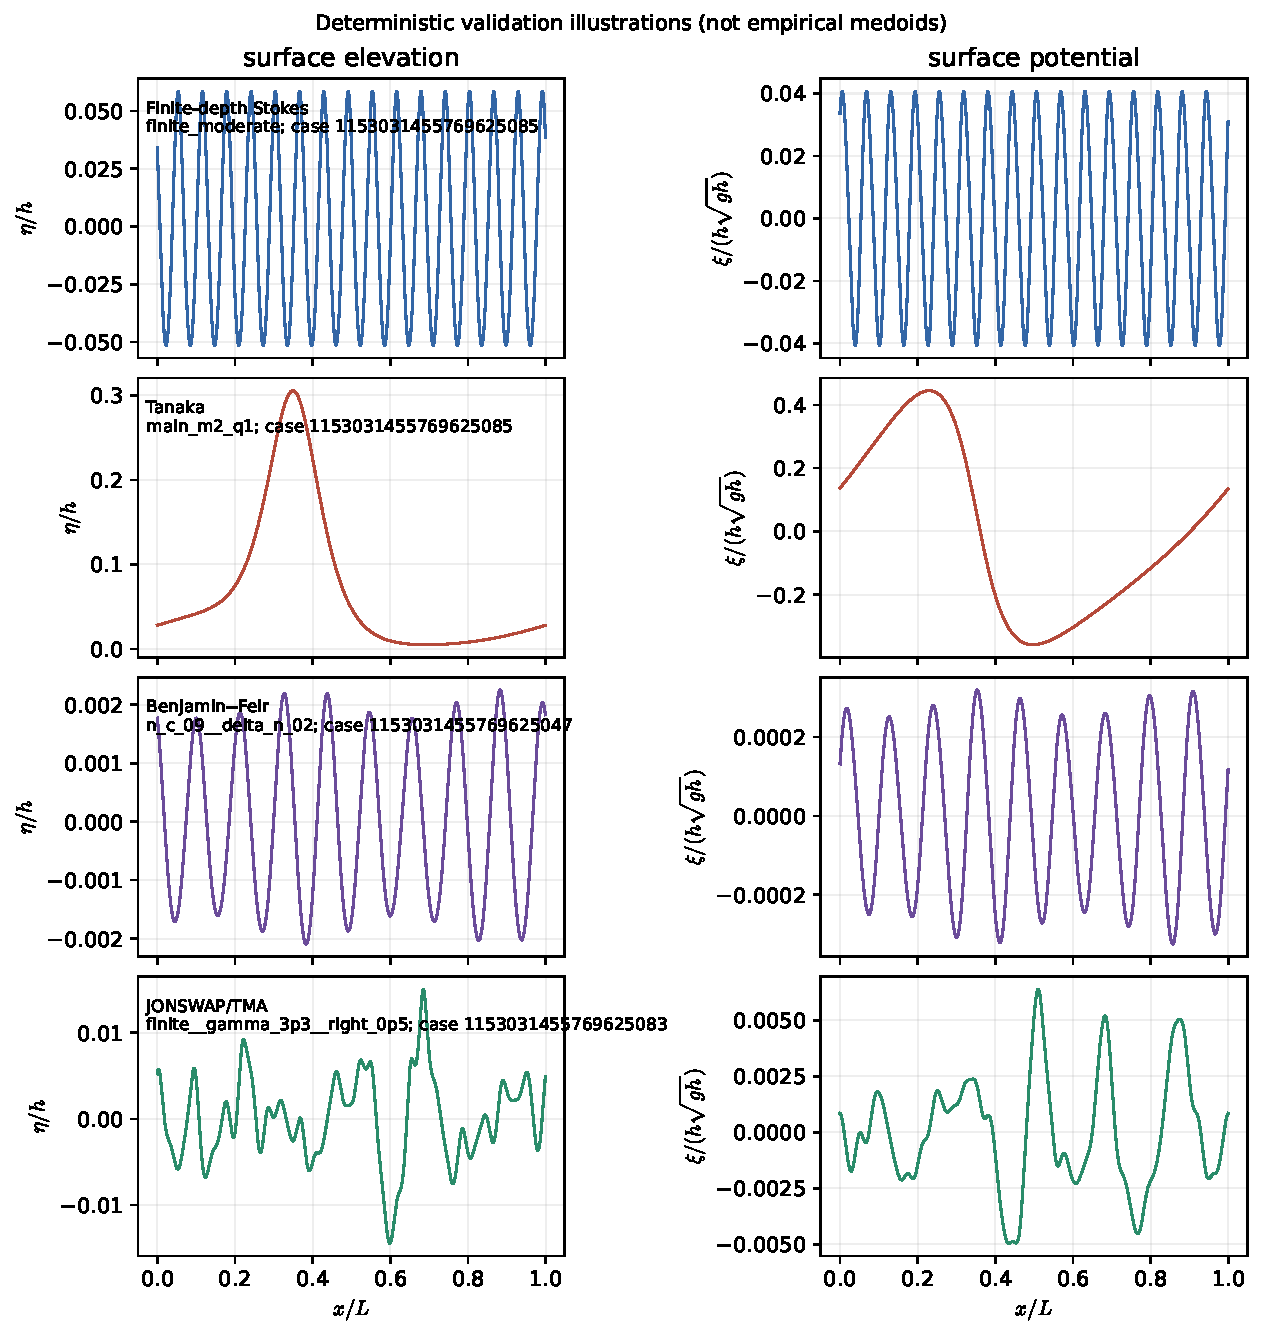
\includegraphics[width=\textwidth]
    {../figures/parameterized_dataset_case_examples.pdf}
  \caption{Deterministic illustrations from accepted validation cases in one
  declared central category per family, selected by the lower-median case ID;
  they are not empirical medoids.  The rows are Stokes revision~2 case
  1153031455769625085 (\texttt{finite\_moderate}), Tanaka revision~3 case
  1153031455769625085 (\texttt{main\_m2\_q1}), Benjamin--Feir revision~4
  case 1153031455769625047 (\texttt{n\_c\_09\_\_delta\_n\_02}), and
  JONSWAP/TMA revision~4 case 1153031455769625083
  (\texttt{finite\_\_gamma\_3p3\_\_right\_0p5}).  Each panel shows the
  first retained row; the left column is \(\eta/h\) and the right column is
  \(\xi/(h\sqrt{gh})\), with \(g=1\).}
  \label{fig:family-examples}
\end{figure}
\FloatBarrier

\section{One numerical rollout and one whole-trajectory decision}
\label{sec:rollout}

Stokes cases are static.  Let $F$ denote one of the three trajectory
families.  The current internal grid size, cutoff, and DNO-series order are
\[
  (N_F,K_F)=
  \begin{cases}
    (1024,256),&F=\text{Tanaka or Benjamin--Feir},\\
    (2048,704),&F=\text{JONSWAP/TMA},
  \end{cases}
\]
and
\[
  M_F=
  \begin{cases}
    6,&F=\text{Tanaka},\\
    4,&F=\text{Benjamin--Feir or JONSWAP/TMA}.
  \end{cases}
\]
This definition applies only to the three rollout families.  Static Stokes
has no evolution cutoff because it is not time-integrated; its single stored
label nevertheless uses the common delivered \(P_{128}\) target in
\eqref{eq:reference-target}.
The unprojected internal DNO output is
\[
  \widetilde G_F(\eta;h)\xi
  =
  \mathcal G_{M_F}^{N_F,8}
    (P_{K_F}\eta;h)(P_{K_F}\xi),
  \qquad
  G_{\mathrm{evol},F}(\eta;h)\xi
  =P_{K_F}^{\circ}\!\left[\widetilde G_F(\eta;h)\xi\right].
\]
The discrete Zakharov equations used for the rollout are
\begin{align}
  \eta_t
  &=
  G_{\mathrm{evol},F}(\eta;h)\xi, \notag\\
  \xi_t
  &=
  P_{K_F}^{\circ}\!\left[
    -\eta-\frac12\xi_x^2
    +\frac{
      \bigl(\widetilde G_F(\eta;h)\xi+\eta_x\xi_x\bigr)^2
    }{2(1+\eta_x^2)}
  \right].
  \label{eq:zakharov}
\end{align}
The Zakharov surface formulation and the Craig--Sulem expansion follow the
formulation used by Xu and Guyenne~\cite{xu2009}.  The truncation order,
spatial grid, padding factor, and delivered Fourier band in this note are
fixed project choices.
The Craig--Sulem calculation inside $\widetilde G_F$ uses padding factor
eight.  Its unprojected value enters the quadratic term before the complete
$\xi_t$ right-hand side is projected.  The products written explicitly in the
second line of \eqref{eq:zakharov} are
formed on a separate two-times Fourier grid before projection.

The linear gravity-wave part of \eqref{eq:zakharov} is advanced exactly in
Fourier space.  More precisely, write the right-hand side as
$L_hz+R_h(z)$, where $z=(\eta,\xi)$, $L_hz$ is the linear part, and $R_h(z)$
is the nonlinear remainder.  A Benjamin--Feir case starts this autonomous
equation immediately.  A JONSWAP/TMA case first solves the
Dommermuth-adjusted equation~\cite{dommermuth2000}
\begin{equation}
  z_t=L_hz+A(t)R_h(z),
  \qquad
  A(t)=1-\exp\!\left[-\left(\frac{t}{10T_p}\right)^4\right].
  \label{eq:jonswap-adjustment}
\end{equation}
Dommermuth supplies the ramped-nonlinearity construction; the exponent four,
the scale $10T_p$, and the $20T_p$ handoff horizon are fixed project
settings validated below rather than unique prescriptions of that method.
until
\begin{equation}
  T_{\mathrm{adj}}
  =0.08\left\lfloor\frac{20T_p}{0.08}\right\rfloor.
  \label{eq:jonswap-adjustment-time}
\end{equation}
This is the last saved-grid time not exceeding $20T_p$.  The complete
2048-point, $K_F=704$ endpoint is handed to the autonomous equation without projection
to $P_{128}$ and without rescaling either component.  At that handoff the
production clock is restarted at zero and $A$ is fixed to one.

For either equation, the change of variable
$v(t)=e^{-tL_h}z(t)$ gives
\[
  v_t=e^{-tL_h}R_h(e^{tL_h}v).
\]
During adjustment, the right-hand side is additionally multiplied by $A(t)$.
The program applies the two-stage, fourth-order Gauss--Legendre method
(GL2) to this transformed equation.  This is the integrating-factor GL2
method described by Xu and Guyenne~\cite{xu2009}.  The step, iteration cap,
and residual test below are our fixed implementation settings.

The GL2 step is $0.01$.  At each step it solves two coupled internal stage
equations.  JONSWAP/TMA permits at most five simultaneous fixed-point updates;
Tanaka and Benjamin--Feir permit at most four.  For each stage and each field
separately, the remaining stage-equation mismatch is divided by the
larger of the stage norm, the fixed-point-map norm, and the smallest normal
floating-point number.  The largest of these relative mismatches must be at
most $10^{-8}$.  After each Tanaka step, the program multiplies every retained
Fourier coefficient of both state fields by
\begin{equation}
  \sigma_k
  =\exp\!\left[-36\left(\frac{|k|}{256}\right)^{36}\right].
  \label{eq:tanaka-hou-li}
\end{equation}
Benjamin--Feir uses the sharp cutoff $|k|\leq256$, while JONSWAP/TMA uses the
sharp cutoff $|k|\leq704$ on 2048 points.  After each completed GL2 step,
both state fields are sharply projected to $P_{256}$ or $P_{704}$,
respectively.  These repeated projections enforce the declared Galerkin
space, but they are not Hou--Li filters and do not smoothly damp the retained
modes.  A candidate state is stored every $0.08$, exactly
every eight steps; there is no time interpolation.  Every delivered state is
projected to $P_{128}$, and its label is then evaluated by the common
order-six formula \eqref{eq:reference-target}.  Thus modes above 128 and, for
Benjamin--Feir and JONSWAP/TMA, the order-four DNO are numerical workspace for
evolution, not additional model inputs or outputs.
For Tanaka, the exact revision-3 chain is: construct and sharply project the
initial state to \(P_{128}\), zero-fill it into \(K_F=256\), apply
\eqref{eq:tanaka-hou-li} to both state fields after every GL2 step, and expose
only the \(P_{128}\) state and common \(P_{128}\) target.  Benjamin--Feir and
JONSWAP/TMA use the same delivered band but their distinct sharply projected,
order-four internal grids and cutoffs stated above.

The step \(0.01\) was selected before production on a fixed historical
revision-2 12-case panel.
All ten cases that completed at both steps \(0.01\) and \(0.005\) agreed to
at most \(1.126337\times10^{-5}\); the other two became incomplete under
both steps.  The \(0.005\) calculation is retained as method-level time-step
evidence, not as a second rollout applied to each production case or as
current-revision population evidence for any family.

Tanaka requests $0\leq t\leq200$.  Benjamin--Feir requests the
case-dependent time $T_{\mathrm{BF}}$ defined above.  After adjustment, a
random sea requests the last $0.08$-grid time no later than $16T_p$.  Its
autonomous time coordinate starts from zero at the full-band handoff.  Cases with
different random-sea horizons may share a numerical batch, but each one is
judged only on its own requested prefix.

Suppose the initial condition already obeys its family's parameter rules.
There is then one trajectory decision:
\begin{equation}
  \boxed{\text{accept}
    \quad\Longleftrightarrow\quad
    \text{the fixed method returns one complete admissible trajectory}.}
  \label{eq:trajectory-acceptance}
\end{equation}
Here \emph{complete admissible trajectory} means that the calculation reaches
its requested final time, every GL2 stage has finite relative residual at
most \(10^{-8}\), every stage and updated state is finite, all saved
\(\eta\), \(\xi\), and \(\Gref(\eta;h)\xi\) values are finite, and
\[
  h+\eta(x_\ell,t_j)>0
\]
at every saved time \(t_j\) and grid point \(x_\ell\).  The final inequality
is the elementary geometric requirement that the graph of the free surface
remain above the flat bottom \(y=-h\).  It has already been checked at
\(t=0\) while assembling the initial batch and is checked again on every
saved state.  The recorded diagnostics state which clause failed; they are
not additional fitted filters.  A failed trajectory
contributes zero rows.  Keeping its finite prefix would systematically give
difficult cases only their earlier, easier states.

Benjamin--Feir revision 4 and JONSWAP/TMA revision 4 cases have one additional numerical
condition.  On every saved frame of their autonomous trajectory, before
projection to $P_{128}$, use $K_F=256$ for Benjamin--Feir and $K_F=704$ for
JONSWAP/TMA and define
\begin{equation}
  H_F(t_j)
  =\frac12\int_0^{2\pi}
    \left\{\xi\,G^{K_F}_4(\eta;h)\xi+g\eta^2\right\}\,\dd x,
  \qquad
  d_{H,F}
  =\max_j\frac{|H_F(t_j)-H_F(0)|}
                   {\max\{|H_F(0)|,\varepsilon_{64}\}},
  \label{eq:internal-hamiltonian}
\end{equation}
where $G^{K_F}_4$ is the order-four DNO evaluated from the full sharp
internal state and $\varepsilon_{64}$ is the smallest positive normal
float64 number.  These cases require
\begin{equation}
  d_{H,F}\leq10^{-3}.
  \label{eq:internal-hamiltonian-limit}
\end{equation}
At the same saved frames the executor records whether the internal state and
$G^{K_F}_4(\eta;h)\xi$ are finite and records the minimum value of
$h+\eta$.  It persists these indicators, the initial Hamiltonian, the maximum
drift, and the minimum water column with the case.  For JONSWAP/TMA,
$H_F(0)$ is computed after the full-band handoff.  Equation
\eqref{eq:internal-hamiltonian-limit} is not imposed during
\eqref{eq:jonswap-adjustment}, because the ramp makes that equation explicitly
time dependent; finiteness, positive water depth, and solved implicit stages
are still required during adjustment.

Only the declared $\Delta t=0.01$ path is run for each production case.  A
failure owns zero rows and is replaced from the same parameter category.
Sign changes, slope, extrema, spectrum, absolute target size, visual
appearance, and model error do not decide acceptance.  Hamiltonian drift
decides acceptance only through
\eqref{eq:internal-hamiltonian-limit} for the two stated families.

A static Stokes state has no trajectory.  It is kept only when its sampled
parameters obey the Stokes rules, its state and common target are finite, and
$h+\eta_0>0$ at every grid point.

\subsection{Why the JONSWAP/TMA cutoff is 704}

The predeclared shallow sentinel used the earlier revision-3 spectral
constructor and was adjusted and evolved independently at two sharp cutoffs
on the 2048-point grid.  The \(K=704\) and \(K=768\) arms used the numerical
method inherited by revision 4.  Over the 16-peak-period autonomous history,
their largest relative whole-field differences were
\begin{equation}
  (e_\eta,e_\xi,e_{G\xi})
  =(4.64267,1.93035,7.91931)\times10^{-4}.
  \label{eq:jonswap-final-cutoff-errors}
\end{equation}
The target in this comparison was recomputed after the normalized transfer in
\eqref{eq:normalized-grid-transfer}; the internal order-four DNO output was
not resampled.  All three values in
\eqref{eq:jonswap-final-cutoff-errors} are below \(10^{-3}\).  The corresponding
\(K=640\) versus \(K=768\) comparison exceeded \(10^{-3}\), so 640 is not the
production cutoff.  Diagnostics formed only from modes
\(96\le|k|\le128\) were about \(3\times10^{-3}\).  The conclusion is therefore
only a global whole-field statement, not a bandwise convergence statement.
Some stage residuals are close to the required \(10^{-8}\), and this is one
worst-case sentinel.  It therefore did not replace a gate using the current
constructor; the revision-4 gate has since passed as reported in
Section~\ref{sec:release}.

The then-current revision-3 source was replayed from the archived full internal
\(K=704\) endpoint.  It reproduced all 289 autonomous saved frames with
maximum relative \(L^2\) errors
\((3.99\times10^{-16},4.66\times10^{-16},1.17\times10^{-15})\) in
\((\eta,\xi,G(\eta)\xi)\).  The replay was accepted, solved every stage, had
maximum residual \(9.994198\times10^{-9}\), Hamiltonian drift
\(1.831187\times10^{-5}\), minimum water column \(0.0387699\), and CPU wall
time 197.355 seconds.  This verifies that historical source and the inherited
evolution method against the archived sentinel; it does not validate the
revision-4 relative-frequency population.

\subsection{Endpoint diagnostics that do not reject cases}
\label{sec:endpoint-diagnostics}

Spatial roughness and sign changes were used historically to find cases that
merited inspection; neither quantity decides acceptance.  We applied two
such rankings to the revision-2 method-level rollout panel.  We first removed the
two trajectories that did not reach their requested terminal time, exactly as
the dataset rule requires.  For the figures below, we then omit the three
JONSWAP/TMA cases because their intentionally broadband spectra otherwise
dominate both rankings and obscure comparison among the coherent-wave
families.  This second omission is only a presentation choice; it does not
remove any case from the dataset.  The displayed rankings therefore use five
completed Tanaka and Benjamin--Feir endpoints.  No last-finite frame from an
incomplete trajectory participates.

Let $\widehat\eta_k$ be the Fourier coefficients of an endpoint elevation
after removal of its mean.  Define its root-mean-square wavenumber by
\begin{equation}
  k_{\mathrm{eff}}(\eta)
  =
  \left(
    \frac{\sum_{k\ne0}k^2|\widehat\eta_k|^2}
         {\sum_{k\ne0}|\widehat\eta_k|^2}
  \right)^{1/2}.
  \label{eq:effective-wavenumber}
\end{equation}
This is large when a substantial fraction of the elevation energy lies at
short spatial scales; by convention it is zero when the denominator
vanishes.  Figure~\ref{fig:terminal-roughness} shows all five completed
non-JONSWAP/TMA cases in decreasing order.

\begin{figure}[ht]
  \centering
  \includegraphics[width=\textwidth]{../../outputs/paper_dataset_terminal_diagnostics_20260726/top_non_jonswap_terminal_spatial_roughness.pdf}
  \caption{Historical revision-2 method-panel cases with the largest endpoint value of
  $k_{\mathrm{eff}}(\eta)$.  In each row, the dashed gray curve is the initial
  field, the colored curve is the terminal field, and the right panel shows
  the corresponding normalized Fourier amplitudes.  Every displayed
  trajectory completed its requested interval, and JONSWAP/TMA cases are
  omitted from this display.  The narrow Tanaka case has the largest value,
  $k_{\mathrm{eff}}=37.52$; spatial roughness alone is therefore not evidence
  of numerical failure.}
  \label{fig:terminal-roughness}
\end{figure}

For the second ranking, let
$f_\ell=[\Gref(\eta;h)\xi](x_\ell)$ at the endpoint and form the cyclic
forward differences
\[
  d_\ell=f_{\ell+1}-f_\ell,\qquad
  \ell=0,\ldots,1023,\qquad f_{1024}=f_0.
\]
Set $\tau=0.03\max_\ell|d_\ell|$, discard differences with
$|d_\ell|\leq\tau$, and count cyclic transitions between the signs of the
remaining differences.  Denote this count by
$C_{0.03}(\Gref(\eta;h)\xi)$.  The dead zone prevents roundoff-sized
differences from creating sign changes.  Figure~\ref{fig:terminal-signs}
shows all five completed non-JONSWAP/TMA cases.

\begin{figure}[ht]
  \centering
  \includegraphics[width=\textwidth]{../../outputs/paper_dataset_terminal_diagnostics_20260726/top_non_jonswap_terminal_sign_changes.pdf}
  \caption{Historical revision-2 method-panel cases with the largest endpoint
  sign-change count in the cyclic
  forward difference of $\Gref(\eta;h)\xi$, after incomplete trajectories
  and the broadband JONSWAP/TMA display cases have been removed.  The
  completed Tanaka upper-corner and Benjamin--Feir upper-boundary cases lead
  with 48 and 40 changes, followed by the narrow Tanaka case with 18.  The
  count detects small oscillatory contributions but does not by itself show
  that a completed trajectory is numerically unstable, so it is retained only
  as a diagnostic.}
  \label{fig:terminal-signs}
\end{figure}
\FloatBarrier

\section{Selecting times after acceptance}
\label{sec:time-selection}

Time selection reduces storage; it never decides whether a case is accepted
and it never uses model error.  Stokes retains only $t=0$.
Tanaka has 2501 candidate times
\[
  t_j=0.08j,\qquad j=0,\ldots,2500,
\]
and retains exactly 200 distinct times, including both endpoints.

For Tanaka, define the total surface-slope energy
\[
  S_{\mathrm T,j}
  =
  \sum_{\ell=0}^{1023}
  |\eta_x(x_\ell,t_j)|^2
\]
and its discrete time difference
\[
  D S_{\mathrm T,j}
  =
  \begin{cases}
    S_{\mathrm T,1}-S_{\mathrm T,0},&j=0,\\
    (S_{\mathrm T,j+1}-S_{\mathrm T,j-1})/2,&1\leq j\leq2499,\\
    S_{\mathrm T,2500}-S_{\mathrm T,2499},&j=2500.
  \end{cases}
\]
The Tanaka activity is
\[
  A_{\mathrm T,j}
  =
  \frac{|D S_{\mathrm T,j}|}
       {S_{\mathrm T,j}+10^{-12}}.
\]
Thus extra weight is given to times when the
surface shape changes rapidly.

The Tanaka activity is smoothed by a fixed Gaussian in the time index.  Its
standard deviation is 50 candidate times.  The kernel stops at three standard
deviations, and values beyond either endpoint are replaced by that endpoint
value.  If $\widetilde A_{\mathrm T,j}$ is the smoothed activity, the
selection weights are
\[
  p_{\mathrm T,j}
  =
  \frac{1-\alpha_{\mathrm T}}{2501}
  +
  \alpha_{\mathrm T}
  \frac{\widetilde A_{\mathrm T,j}}
       {\sum_{r=0}^{2500}\widetilde A_{\mathrm T,r}},
  \qquad \alpha_{\mathrm T}=0.50.
\]
If all activities vanish, the second term is replaced by a uniform weight.
The program takes fixed midpoint quantiles of the cumulative weights, pins
the first and last times, and clips each quantile index so that enough unused
indices remain for all later quantiles.  A forward pass then advances any
repeated index to the next unused one.  The result is deterministic.

For Benjamin--Feir, let $J_{\mathrm{BF}}=T_{\mathrm{BF}}/0.08$.  Store the
200 indices
\[
  j_\ell
  =\left\lfloor\frac{\ell J_{\mathrm{BF}}}{199}+\frac12\right\rfloor,
  \qquad \ell=0,\ldots,199.
\]
These indices are approximately uniform in time and include both endpoints.
Thus the storage rule introduces no additional event score beyond the
declared 100-carrier-period horizon.

For a random sea, let
\[
  T_s=0.08\left\lfloor\frac{16T_p}{0.08}\right\rfloor,
  \qquad J_s=T_s/0.08.
\]
It retains the 16 indices
\[
  j_\ell=
  \left\lfloor\frac{\ell J_s}{15}+\frac12\right\rfloor,
  \qquad \ell=0,\ldots,15.
\]
These are approximately uniform and include $0$ and $T_s$.  Here $t=0$ is
the adjusted full-band endpoint and the start of autonomous production, not
the initial linear random sea.

\section{Identity, splitting, quotas, and storage}
\label{sec:records}

\subsection{Case identity and data splits}

The full case identity consists of
\[
  (\text{family},\ \text{revision},\ \text{split},\
    \text{stream},\ \text{attempt}).
\]
Its deterministic random stream instead uses these five integer seed words:
\[
  (\text{split root},\ \text{family},\ \text{revision},\
    \text{stream},\ \text{attempt}).
\]
These words seed NumPy's PCG64 generator.  The split roots are
\[
  \begin{array}{c|ccc}
    \text{split}&\text{training}&\text{validation}&\text{test}\\ \hline
    \text{root}&2026072210&2026072204&2026072205.
  \end{array}
\]
The split, parameter category, and entire sampled specification are written
before construction or integration.  A rejection remains attached to that
split.  All stored times from one trajectory therefore stay together, so
nearby times from the same numerical solution cannot cross into validation
or test.

\subsection{Accepted-case quotas}

A quota is a required number of accepted complete cases, not a number of
attempts or stored rows.  Suppose a family has $m$ ordered parameter
categories and requires $C$ accepted cases.  Write
\[
  C=bm+r,\qquad 0\leq r<m.
\]
The first $r$ categories receive $b+1$ cases and the other categories receive $b$.
This is the most even integer division possible.

A failed attempt is replaced only in its original category.  A category assigned
$Q$ accepted cases may use at most $4Q$ recorded attempts.  If the
resolved attempts reach this bound without filling $Q$, the family run stops
as incomplete.  Another category cannot fill the deficit.  The factor four
only bounds computation; it does not change any case-level decision.  The
Stokes amplitude redraws described above are internal to one attempt.

The family sampling formulas govern attempted specifications, not the
unconditional law of loader-visible cases.  If \(X\) is a complete attempted
specification in preassigned category \(i\), \(A_f\) is the declared complete
case-acceptance event for family \(f\), and \(w_i\) is the accepted-quota
weight, then
\[
  p_{\mathrm{release}}(i,x)
  =w_i\,p_{\mathrm{proposal}}(x\mid i,A_f=1).
\]
For Stokes, \(A_f\) comprises declared static support, a finite state, positive
water column, and a finite target.  For Tanaka, it comprises declared
construction support followed by complete autonomous-trajectory acceptance;
for Benjamin--Feir, initial-state validity followed by complete autonomous-
trajectory acceptance.  For JONSWAP/TMA, it comprises initial construction and
graph validity followed by nonlinear adjustment and complete autonomous-
trajectory acceptance.  Consequently the quota preserves the declared
category marginals, not the unconditioned proposal law within a category.
This identity describes release construction; it does not by itself claim a
measured within-category shift for every family.  Every rejected proposal
remains recorded, and no retrospective parameter cutoff is applied.

\subsection{Files and combined view}

An accepted row stores three length-1024 spatial arrays
$\eta$, $\xi$, and $\Gref(\eta;h)\xi$ in float32, together with float64 depth
and time, its selected candidate-time index, and its case-local index in that
array file.
The case record preserves the sampled parameters and numerical decision for
both accepted and rejected attempts.  It also binds the family, split,
random stream, numerical settings, software versions, source hashes, and
array checksum.

After the four families have been generated for all three splits, the
combined builder checks the records, shapes, checksums, and required counts.
It allows exactly one revision for each family.  Source and numerical
settings must agree among all chunks and splits with the same
$(\text{family},\text{revision})$ pair; settings from two different families
are not required to be identical.  This is necessary because Tanaka revision
3 uses 1024 points and internal cutoff 256, Benjamin--Feir revision 4 uses the
same grid and cutoff with a different DNO order, JONSWAP/TMA revision 4 uses
2048 points and cutoff 704, and revision-2 Stokes is static.  The builder then writes
a compact row-to-case index pointing to the existing
arrays rather than copying them.  This index is the dataset view read by the
trainer.

\section{Production size and trainer handoff}
\label{sec:handoff}

The first checkpoint requests, from \emph{each} family,
\[
  2048\ \text{training},\qquad
  1024\ \text{validation},\qquad
  1024\ \text{test cases}.
\]
The four families therefore contain 16,384 accepted cases in total.
For one accepted case from each family, the stored-row count is
\[
  1+200+200+16=417.
\]
The exact split counts are
\begin{table}[ht]
  \centering
  \small
  \begin{tabular}{lrr}
    \toprule
    Split & Accepted cases & Stored rows\\
    \midrule
    Training & 8,192 & 854,016\\
    Validation & 4,096 & 427,008\\
    Test & 4,096 & 427,008\\
    \midrule
    Total & 16,384 & 1,708,032\\
    \bottomrule
  \end{tabular}
\end{table}
The authenticated final view references 1315 physical field shards containing
7686144 rows and 94,666,557,624 measured bytes (88.165102 GiB).  Cumulative
views reference immutable source prefixes and do not copy those fields.
Training then grows by additive, disjoint chunks to
\[
 C_{\mathrm{tr}}\in\{2048,4096,8192,16384\}
\]
accepted cases per family; validation and test remain fixed at 1024 cases per
family.  The resulting cumulative sizes are
\begin{center}
\begin{tabular}{rr}
  \toprule
  Training cases per family & Total stored rows \\
  \midrule
  2,048  & 1,708,032 \\
  4,096  & 2,562,048 \\
  8,192  & 4,270,080 \\
  16,384 & 7,686,144 \\
  \bottomrule
\end{tabular}
\end{center}
Thus 2048 is a checkpoint, not the completed dataset.  The target at 16,384
contains 73,728 accepted cases across the four families and three splits.
Its 7,686,144 rows are close to the 7,633,989 rows in historical v9: 52,155
more rows, or 0.68\%.

Normalization is computed from all stored \emph{training} rows and from no
validation, test, or diagnostic rows.  Let $\eta_i$, $\xi_i$, and $h_i$
denote the elevation, potential, and depth in training row $i$, and let
$G_i^\star=\Gref(\eta_i;h_i)\xi_i$ denote its reference label.  Define
\[
  s_\eta=\max_{i,x}|\eta_i(x)|,\qquad
  s_\xi=\max_{i,x}|\xi_i(x)|,\qquad
  s_G=\max_{i,x}|G_i^\star(x)|.
\]
The authenticated training-only values are
\(s_\eta=0.15583430230617523\),
\(s_\xi=0.09394174814224243\), and
\(s_G=0.12198150902986526\), computed from 6832128 rows.  The release audit
verifies all three before training.  The current loader uses one as
a defensive fallback if a nonpositive scale reaches it; that fallback is not
treated as validation of a malformed dataset.  The cached values are tied to
the checked dataset identity; their statistics fingerprint is
\path{4e8ec96947bc05cee3b375467499b0ae00a7814f9982614084efd859efe7c3b8}.
The trainer receives
\[
  \eta/s_\eta,\qquad
  \xi/s_\xi,\qquad
  \log(h/h_\star),\qquad
  \Gref(\eta;h)\xi/s_G,
\]
where the reference length is $h_\star=L/(2\pi)=1$ on the production domain.
The paper-dataset training command must explicitly select this scale
normalization with \texttt{--norm scale}; the trainer's generic min--max
default is not the rule stated here.

At every training epoch, the loader chooses one stored time uniformly from
every accepted training case.  Thus each family contributes
$C_{\mathrm{tr}}$ samples per epoch even though the archive stores different
numbers of times per case.  Validation uses one fixed deterministic time per
case.  Airy,
manufactured-DNO, and sparse-Fourier states remain diagnostic tests and do
not enter training or its normalization.

\section{Checks before bulk generation}
\label{sec:release}

Grid, truncation, padding, spectral support, and time step are chosen on
fixed method-level panels before bulk generation.  They are not re-estimated
for individual production cases.  The current family-specific checks are not
one mixed numerical batch.  The Tanaka revision-3 pilot used complementary
six- and five-case shards and passed: all 11 attempted cases were accepted,
none was rejected, and the accepted trajectories produced 2200 rows.  The
artifacts carry validation split tags so that the transaction path is tested,
but their dedicated pilot roots are diagnostic and are excluded from final
validation data, training, and normalization.  This establishes the eleven
Tanaka categories only; it is not part of corrected bulk production.

The revision-4 Benjamin--Feir production-law gate used stream 935.  It
accepted all 66 first proposals, rejected none, and retained 13,200 rows.
Over its accepted cases,
the largest implicit-stage residual was $9.999967\times10^{-9}$, the largest
relative internal-Hamiltonian drift was $2.952009\times10^{-5}$, and the
smallest water column was $4.960598$.  The earlier stream-934 result remains
independent support-validation evidence; stream 935 is the direct revision-4
production gate.

A preceding revision-3 JONSWAP/TMA source gate used stream 933.  It accepted
one case in every category after 29 attempts, retained 432 rows, and rejected
two attempts with zero rows.  The first proposals in
\texttt{finite\_\_gamma\_3p3\_\_right\_1} and
\texttt{shallow\_\_gamma\_1\_\_right\_0p5} stopped during nonlinear
adjustment; the canonical second proposal in each category passed.  Among the
27 accepted cases, the corresponding three extrema were
$9.999783\times10^{-9}$, $5.908800\times10^{-5}$, and $0.0127322$.
This gate remains historical evidence for the inherited adjustment and
evolution method; it does not test the revision-4 relative-frequency
constructor.

The independent audit rederived every proposal and run specification and
passed.  Its artifact is
\path{outputs/nondataset_bf_revision4_jonswap_revision3_category_smoke_20260802/category_smoke_release_audit_v1.json},
with SHA-256
\par\noindent
\texttt{62fb5fe3b6be7df0d21784b1ce590c44cc484bf5fdf84ad6097fbed6f655f684}.
This preserves the independent audit of the revision-4 Benjamin--Feir gate
and the historical revision-3 JONSWAP/TMA gate; one case per category does
not estimate a population rejection rate.  The
JONSWAP/TMA \(K=704\) versus \(K=768\) sentinel remains the separate
whole-field cutoff check in \eqref{eq:jonswap-final-cutoff-errors}.  Likewise, the four
static Stokes revision-2 categories passed their own exact calculation, with
all four cases accepted and all failed-quality masks zero.  One case per
category tests construction and evolution.

The direct revision-4 JONSWAP/TMA gate fixed 20 accepted cases in each of the
27 categories before execution.  It retained 540 cases from 548 attempts;
eight incomplete numerical attempts retained zero rows.  The observed
rejection rate was \(1.46\%\), below the predeclared two-percent bound.  This
is the current-constructor gate used before revision-4 bulk generation, not a
bulk release threshold.  Its
audited summary is
\path{outputs/jonswap_relative_band_fresh_gate_20260804/jonswap_relative_band_fresh_gate.summary.json}.

A family's bulk generation began only after its own current-source check
passed.  The final release audit then checked exact case and row counts,
disjoint splits, finite stored arrays, positive depths, zero-row failed cases,
checksums, and training-only normalization.

\paragraph{Final authenticated status.}
All four family revisions are complete at 16384 training, 1024 validation,
and 1024 test cases each.  Stokes retained 18432 cases from 18432 attempts and
stored 18432 rows; corrected Tanaka retained 18432/18432 and stored 3686400
rows; Benjamin--Feir retained 18432/18455 and stored 3686400 rows; and
JONSWAP/TMA retained 18432/18726 and stored 294912 rows.  Thus the release has
73728 accepted cases from 74045 attempts, 317 zero-row rejections, and
7686144 rows.  The combined rejection rate is \(0.428118\%\).  The
historical 4096-case Tanaka population and all diagnostic gates remain outside
the release.

The cumulative combined-summary SHA-256 identities for 2048, 4096, 8192, and
16384 training cases per family are, respectively:
\begin{center}
\small
\texttt{2265cb71270accb3f6d9103e90433b664ca813989dfab63403d8612af22d28c3}\\
\texttt{7feb018ee4d94eab10278917c145262026cccab6169eaaa2d8877f7c7b28c9da}\\
\texttt{43b1eb91198e724c6f32b871c2d0efd0d8355533789919df5897ad588e7e85f6}\\
\texttt{32f764cf865c90892ee0329e48fe992cbc24df2707e05fd1af2ee9cd2b84307c}.
\end{center}
The final 26-source manifest and trajectory-map SHA-256 identities are
\begin{center}
\small
\texttt{dbb76ed1cba4d0146f3c9643a73d168d3a9fa97bc27c37fe0fd7ad08554bd734}\\
\texttt{f26888ad0a2c738405fb1662b9410337e1babfe48f7913805b5243ae0f279cc8}.
\end{center}
The immutable document handoff has SHA-256
\begin{center}
\small
\texttt{b21830cf56f9c17a1ee165624c71fdc0e286727747d364330fbace19e5ef6053}.
\end{center}
No reported model has been trained on this replacement dataset.

{\footnotesize
\begin{thebibliography}{99}
\setlength{\itemsep}{0pt}

\bibitem{fenton1985}
J.~D. Fenton,
\newblock A fifth-order Stokes theory for steady waves,
\newblock \emph{Journal of Waterway, Port, Coastal, and Ocean Engineering}
111(2) (1985), 216--234.

\bibitem{zhao2024}
K.~Zhao, Y.~Wang, and P.~L.-F. Liu,
\newblock A guide for selecting periodic water wave theories,
\newblock \emph{Coastal Engineering} 188 (2024), 104432.

\bibitem{xu2009}
L.~Xu and P.~Guyenne,
\newblock Numerical simulation of three-dimensional nonlinear water waves,
\newblock \emph{Journal of Computational Physics} 228 (2009), 8446--8466,
\newblock doi:10.1016/j.jcp.2009.08.015.

\bibitem{tanaka1986}
M.~Tanaka,
\newblock The stability of solitary waves,
\newblock \emph{Physics of Fluids} 29(3) (1986), 650--655,
\newblock doi:10.1063/1.865459.

\bibitem{benjaminfeir1967}
T.~B. Benjamin and J.~E. Feir,
\newblock The disintegration of wave trains on deep water. Part 1. Theory,
\newblock \emph{Journal of Fluid Mechanics} 27(3) (1967), 417--430,
\newblock doi:10.1017/S002211206700045X.

\bibitem{dommermuth1987}
D.~G. Dommermuth and D.~K.~P. Yue,
\newblock A high-order spectral method for the study of nonlinear gravity
waves,
\newblock \emph{Journal of Fluid Mechanics} 184 (1987), 267--288,
\newblock doi:10.1017/S002211208700288X.

\bibitem{andrade2023}
D.~Andrade and R.~Stuhlmeier,
\newblock The nonlinear Benjamin--Feir instability---Hamiltonian dynamics,
discrete breathers and steady solutions,
\newblock \emph{Journal of Fluid Mechanics} 958 (2023), A17,
\newblock doi:10.1017/jfm.2023.96.

\bibitem{yangliu2024}
Z.~Yang and P.~L.-F. Liu,
\newblock New 2-D horizontal free-surface-flow models with applications for
water waves,
\newblock \emph{Journal of Fluid Mechanics} 999 (2024), A32,
\newblock doi:10.1017/jfm.2024.604.

\bibitem{dommermuth2000}
D.~G. Dommermuth,
\newblock The initialization of nonlinear waves using an adjustment scheme,
\newblock \emph{Wave Motion} 32(4) (2000), 307--317,
\newblock doi:10.1016/S0165-2125(00)00047-0.

\bibitem{hasselmann1973}
K.~Hasselmann et al.,
\newblock Measurements of wind-wave growth and swell decay during the Joint
North Sea Wave Project (JONSWAP),
\newblock \emph{Erg\"anzungsheft zur Deutschen Hydrographischen Zeitschrift},
Reihe A(8), No.~12, 1973.

\bibitem{bouws1985}
E.~Bouws, H.~G\"unther, W.~Rosenthal, and C.~L. Vincent,
\newblock Similarity of the wind wave spectrum in finite depth water:
1. Spectral form,
\newblock \emph{Journal of Geophysical Research: Oceans} 90(C1) (1985),
975--986,
\newblock doi:10.1029/JC090iC01p00975.

\bibitem{grice2015}
J.~R. Grice, P.~H. Taylor, and R.~Eatock Taylor,
\newblock Second-order statistics and `designer' waves for violent
free-surface motion around multi-column structures,
\newblock \emph{Philosophical Transactions of the Royal Society A} 373(2033)
(2015), 20140113,
\newblock doi:10.1098/rsta.2014.0113.

\bibitem{draycott2026}
S.~Draycott, X.~Li, Q.~Xiao, and P.~Stansby,
\newblock Modelling irregular nonlinear waves: potential flow and
volume-of-fluid comparison with experiment,
\newblock \emph{Journal of Ocean Engineering and Marine Energy} (2026),
\newblock doi:10.1007/s40722-026-00495-0.

\bibitem{ducrozet2017applicability}
G.~Ducrozet, F.~Bonnefoy, and Y.~Perignon,
\newblock Applicability and limitations of highly non-linear potential flow
solvers in the context of water waves,
\newblock \emph{Ocean Engineering} 142 (2017), 233--244,
\newblock doi:10.1016/j.oceaneng.2017.07.003.

\bibitem{ducrozet2021rogue}
G.~Ducrozet, M.~Abdolahpour, F.~Nelli, and A.~Toffoli,
\newblock Predicting the occurrence of rogue waves in the presence of
opposing currents with a high-order spectral method,
\newblock \emph{Physical Review Fluids} 6 (2021), 064803,
\newblock doi:10.1103/PhysRevFluids.6.064803.

\end{thebibliography}
}

\end{document}
